\newpage


\section{Dados do Problema}

\subsection{Geometria da Viga}
A viga analisada apresenta os seguintes parâmetros geométricos:
\begin{itemize}
    \item \textbf{Largura} (\( b \)): \(30 \text{ cm} = 0.30 \text{ m}\)
    \item \textbf{Altura} (\( h \)): \(100 \text{ cm} = 1.00 \text{ m}\)
    \item \textbf{Comprimento do trecho analisado}: \( c = 2 \text{ m}\)
\end{itemize}

O momento de inércia da seção transversal é calculado como:

\begin{equation}
    I = \frac{b h^3}{12} = \frac{(0.30)(1.00)^3}{12} = 0.025 \text{ m}^4
\end{equation}

\subsection{Propriedades do Material}
\begin{itemize}
    \item \textbf{Módulo de elasticidade} (\( E \)): \(200 \times 10^9 \text{ Pa}\)
    \item \textbf{Módulo de elasticidade transversal} (\( G \)): \(80 \times 10^9 \text{ Pa}\)
    \item \textbf{Massa específica} (\( \rho \)): \(2000 \text{ kg/m}^3\)
    \item \textbf{Coeficiente de Poisson} (\( v \)): 0.3
\end{itemize}

\subsection{Carregamentos Aplicados}
A viga está sujeita a:
\begin{itemize}
    \item Forças pontuais:
    \[
        F_1 = -4 \times 10^3 \text{ N}, \quad F_2 = -4 \times 10^3 \text{ N}, \quad F_3 = -12 \times 10^3 \text{ N}
    \]
    \item Carga distribuída móvel:
    \[
        q_{\text{móvel}} = -2 \times 10^3 \text{ N/m}
    \]
    \item Carga distribuída do peso próprio:
    \[
        q_{\text{peso}} = -A_{\text{área}} \times \rho \times g = -0.30 \times 1.00 \times 2000 \times 9.81 = -5880 \text{ N/m}
    \]
\end{itemize}


\section{Cálculo das Reações de Apoio}
O equilíbrio de forças na viga é dado por:

\begin{equation}
    \sum F_y = 0 \Rightarrow R_A + R_B + q_{\text{peso}} (L_{\text{spam1}} + L_{\text{spam2}}) + q_{\text{móvel}} (2c) + F_1 + F_2 + F_3 = 0
\end{equation}

\begin{equation}
    \sum F_x = 0 \Rightarrow R_A + R_B =145720 \text{N}
\end{equation}

Já o equilíbrio de momentos em relação ao ponto \( A \) é expresso como:

\begin{equation}
    \sum M_A = 0 \Rightarrow q_{\text{peso}} \frac{20^2}{2} + q_{\text{móvel}} \frac{(10^2 - 6^2)}{2} + F_1 \times 6 + F_2 \times 7.5 + F_3 \times 9 + R_B \times 16 = 0
\end{equation}

Resolvendo o sistema de equações acima, encontramos os valores das reações de apoio:

\begin{equation}
    R_A = 58020 \text{N}, \quad R_B = 87700\text{N}
\end{equation}


\section{Determinação dos Esforços na Viga}

\subsection{Momento Fletor \( M(x) \)}
A função do momento fletor ao longo da viga é descrita pelas equações de macaulay para cada trecho de interesse, no caso:

\begin{equation}
    M(x) =
    \begin{cases}
        R_A x + \frac{q_{\text{peso}}}{2} x^2, & 0 \leq x < 2 \\
        R_A x + \frac{q_{\text{peso}}}{2} x^2, & 2 \leq x < 6 \\
        R_A x + \frac{q_{\text{peso}}}{2} x^2 + \frac{q_{\text{móvel}}}{2} (x - 6)^2 + F_1 (x - 6) + F_2 (x - 7.5), & 6 \leq x < 8 \\
        R_A x + \frac{q_{\text{peso}}}{2} x^2 + \frac{q_{\text{móvel}}}{2} (x - 6)^2 + F_1 (x - 6) + F_2 (x - 7.5) + F_3 (x - 9), & 8 \leq x < 10 \\
        R_A x + \frac{q_{\text{peso}}}{2} x^2 + \frac{q_{\text{móvel}}}{2} (x - 6)^2 + F_1 (x - 6) + F_2 (x - 7.5) + F_3 (x - 9) \\ - \frac{q_{\text{móvel}}}{2} (x - 10)^2, & 10 \leq x < 12\\
        R_A x + \frac{q_{\text{peso}}}{2} x^2 + \frac{q_{\text{móvel}}}{2} (x - 6)^2 + F_1 (x - 6) + F_2 (x - 7.5) + F_3 (x - 9) \\ - \frac{q_{\text{móvel}}}{2} (x - 10)^2, & 12 \leq x < 14\\
        R_A x + \frac{q_{\text{peso}}}{2} x^2 + \frac{q_{\text{móvel}}}{2} (x - 6)^2 + F_1 (x - 6) + F_2 (x - 7.5) + F_3 (x - 9) \\ - \frac{q_{\text{móvel}}}{2} (x - 10)^2, & 12 \leq x < 14\\
        R_A x + \frac{q_{\text{peso}}}{2} x^2 + \frac{q_{\text{móvel}}}{2} (x - 6)^2 + F_1 (x - 6) + F_2 (x - 7.5) + F_3 (x - 9) \\ - \frac{q_{\text{móvel}}}{2} (x - 10)^2 + R_B (x-16), & 14 \leq x < 16\\
        R_A x + \frac{q_{\text{peso}}}{2} x^2 + \frac{q_{\text{móvel}}}{2} (x - 6)^2 + F_1 (x - 6) + F_2 (x - 7.5) + F_3 (x - 9) \\ - \frac{q_{\text{móvel}}}{2} (x - 10)^2 + R_B (x-16), & 16 \leq x \leq 20\\
    \end{cases}
\end{equation}

\subsection{Força Cortante \( V(x) \)}
O esforço cortante é obtida pela derivada do momento fletor:

\begin{equation}
    V(x) = -\frac{dM}{dx}
\end{equation}

\subsection{Inclinação \( \theta(x) \)}
O ângulo de inclinação é calculado por:

\begin{equation}
    \theta(x) = \int \frac{M(x)}{E I} dx
\end{equation}

\subsection{Deflexão Vertical \( y(x) \)}
A equação de deflexão da viga é obtida integrando o ângulo de inclinação:

\begin{equation}
    y(x) = \int \theta(x) dx
\end{equation}

\subsection{Condições de contorno para cada secção}

\begin{table}[h]
    \centering
    \renewcommand{\arraystretch}{1.5}
    \setlength{\arrayrulewidth}{0.5mm}
    \setlength{\tabcolsep}{8pt}
    \arrayrulecolor{black}
    \rowcolors{2}{gray!20}{white}
    \caption{\textbf{\normalsize 📌 Resumo das Condições Atualizadas}}
    \label{tab:resumo_condicoes}
    \begin{tabular}{>{$}l<{$} | >{$}l<{$} | >{$}l<{$}}
        \toprule \rowcolor{gray!50} \hline
        \textbf{Ponto}                                & \textbf{Esforço Cortante $V(x)$} & \textbf{Momento Fletor $M(x)$} \\
        \midrule\hline
        x = 0m \text{ (apoio simples)}                & V(0) = R_A                       & M(0) = 0                       \\\hline
        x = 6m \text{ (carga pontual } P_1 \text{)}   & V(6^+) = V(6^-) - P_1            & M(6^-) = M(6^+)                \\\hline
        x = 7.5m \text{ (carga pontual } P_2 \text{)} & V(7.5^+) = V(7.5^-) - P_2        & M(7.5^-) = M(7.5^+)            \\\hline
        x = 9m \text{ (carga pontual } P_3 \text{)}   & V(9^+) = V(9^-) - P_3            & M(9^-) = M(9^+)                \\\hline
        x = 16m \text{ (apoio simples)}               & V(16^+) = V(16^-) - R_B          & M(16) = 0                      \\\hline
        \bottomrule
    \end{tabular}
\end{table}

\subsection{Resultados obtidos}
\newpage
\thispagestyle{empty}
\begin{landscape}
    \include{out/nos}
\end{landscape}


\section{Resultados e Gráficos}
Os gráficos a seguir representam os diagramas estruturais da viga:

\begin{figure}[H]
    \centering
    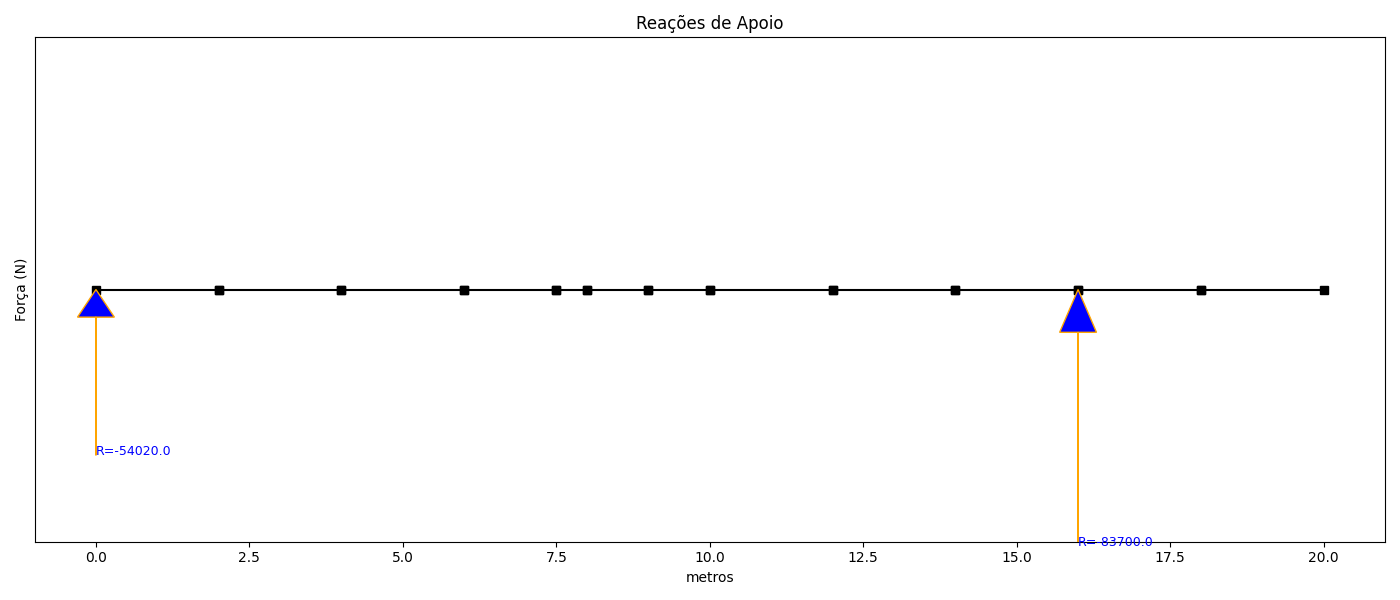
\includegraphics[width=1\textwidth]{images/reacoes}
    \caption{Reações de Apoio}
\end{figure}

\begin{figure}[H]
    \centering
    
\includegraphics[width=1\textwidth]{images/momento}
    \caption{Diagrama de Momento Fletor}
\end{figure}

\begin{figure}[H]
    \centering
    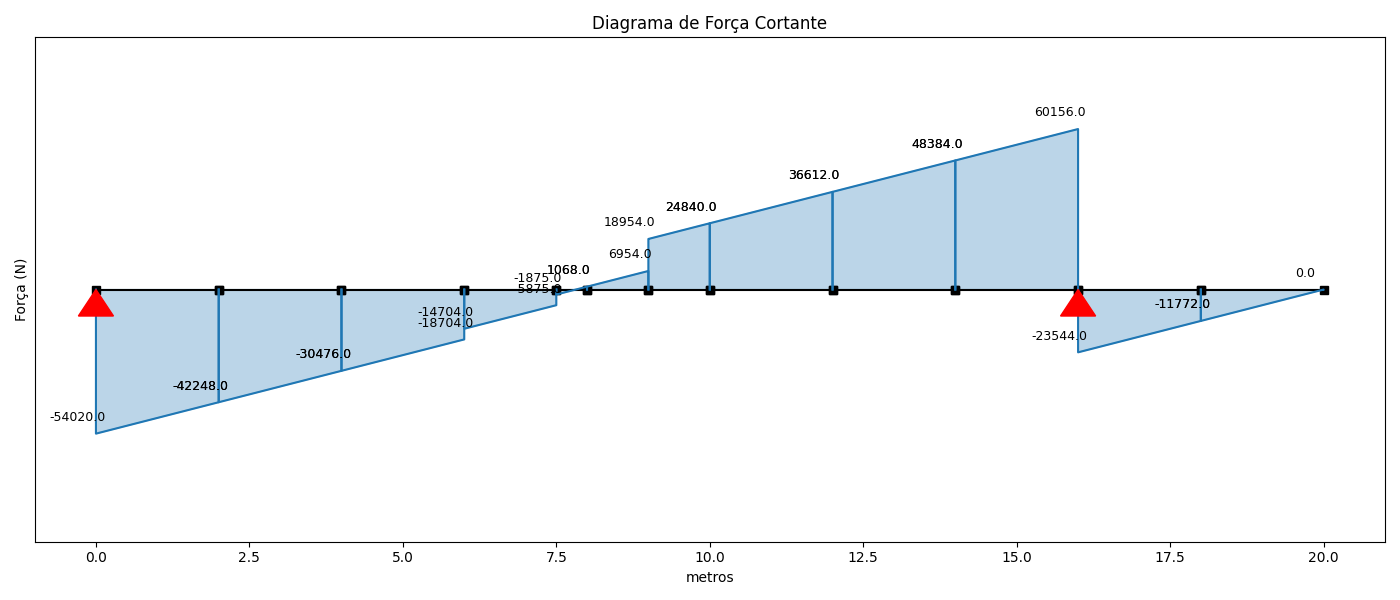
\includegraphics[width=1\textwidth]{images/cortante}
    \caption{Diagrama de Força Cortante}
\end{figure}

\begin{figure}[H]
    \centering
    
\includegraphics[width=1\textwidth]{images/deslocamento}
    \caption{Deformação da Viga}
\end{figure}


\section{Conclusão}
A análise estrutural revelou as distribuições de momento fletor, força cortante e deslocamento ao longo da viga. O método simbólico utilizando Python permitiu calcular as equações dos esforços, garantindo precisão nos resultados.
